\documentclass[12pt]{article}
\usepackage[utf8]{inputenc}
\usepackage{amsmath}
\usepackage{systeme}
\usepackage{amsfonts}
\usepackage{graphicx}
\usepackage{enumitem}
\usepackage{hyperref}
\usepackage{xcolor}
\usepackage{kbordermatrix}
\usepackage{centernot}
\usepackage{xcolor}

\title{%
	\textbf{Notițe Seminar 3}}

\begin{document}
	
	\maketitle
	
	\textbf{\large{Intro}}:
	
	Dacă seminarul trecut am discutat de E și Var că pot fi aplicate pe o variabilă aleatore și că furnizează un număr real, acum vom adăuga la cele două și \textbf{H}-ul.
	
	\textbf{\large{Teoria informației}}
	
	Fie un experiment aleator (de exemplu: aruncăm o monedă). Considerăm că avem următoarea variabilă aleatoare (de exemplu: 0 pentru tails, 1 pentru heads):
	$$X:\begin{pmatrix}
	0 & 1\\
	0.0001 & 0.9999
	\end{pmatrix}$$ 
	În urma experimentului, dorim să observăm valoarea lui $X$. 
	
	Să presupunem că facem experimentul, iar în urma lui, observăm valoarea 0 pentru $X$. 
	
	\newpage
	
	V-am lăsat un moment ca să vă reveniți. Ați rămas surprinși când ați auzit că a ieșit 0, așa-i? De ce? Pentru că $P(X = 0)$ este foarte mică, iar $P(X = 1)$ este foarte mare.
	
	Am putea defini surpriza ca fiind opusul/inversul probabilității. Hai să luăm $\frac{1}{p(x)}$, unde $p$ este pmf-ul lui $X$. Dar hai să-i mai punem și un logaritm în baza 2 în față ca să îl putem măsura în \textbf{biți} (Aceasta este doar o intuiție. Pentru informații formale, dacă vă interesează, vedeți ex. 33/pag. 68):
	$$\text{surpriza}(x) = \log_2\frac{1}{p(x)}$$
	unde $x \in \text{Val}(X)$.
	
	Surpriza poate fi privită și ca variabilă aleatoare:
	$$\text{Surpriza}(X) = \log_2 \frac{1}{p(X)}$$
	unde $X$ este o variabilă aleatoare.
	
	În exemplul nostru, avem:
	$$\text{Surpriza}(X) : \begin{pmatrix}
	\log_2 \frac{1}{0.0001} & \log_2 \frac{1}{0.9999}\\
	0.0001&0.9999
	\end{pmatrix}$$
	
	Haideți să calculăm \textbf{surpriza medie}:
	$$E[\text{Surpriza}(X)] = E[\log_2 \frac{1}{p(X)}] = \log_2 \frac{1}{0.0001} \cdot 0.0001 + \log_2 \frac{1}{0.9999} \cdot 0.9999 = 0.001473...$$
	
	\textbf{Atenție! De obicei, calculatorul științific nu are $\log_2$, ci $\ln$ și/sau $\log_{10}$. Așadar trebuie să amintiți următoarea formulă de schimbare a bazei logaritmului:
		$$\log_2 x = \frac{\ln x}{\ln 2} = \frac{\log_{10} x}{\log_{10} 2}$$}
	
	Surpriza medie se va chema \textbf{entropie}.
	\newpage
	\begin{center}
		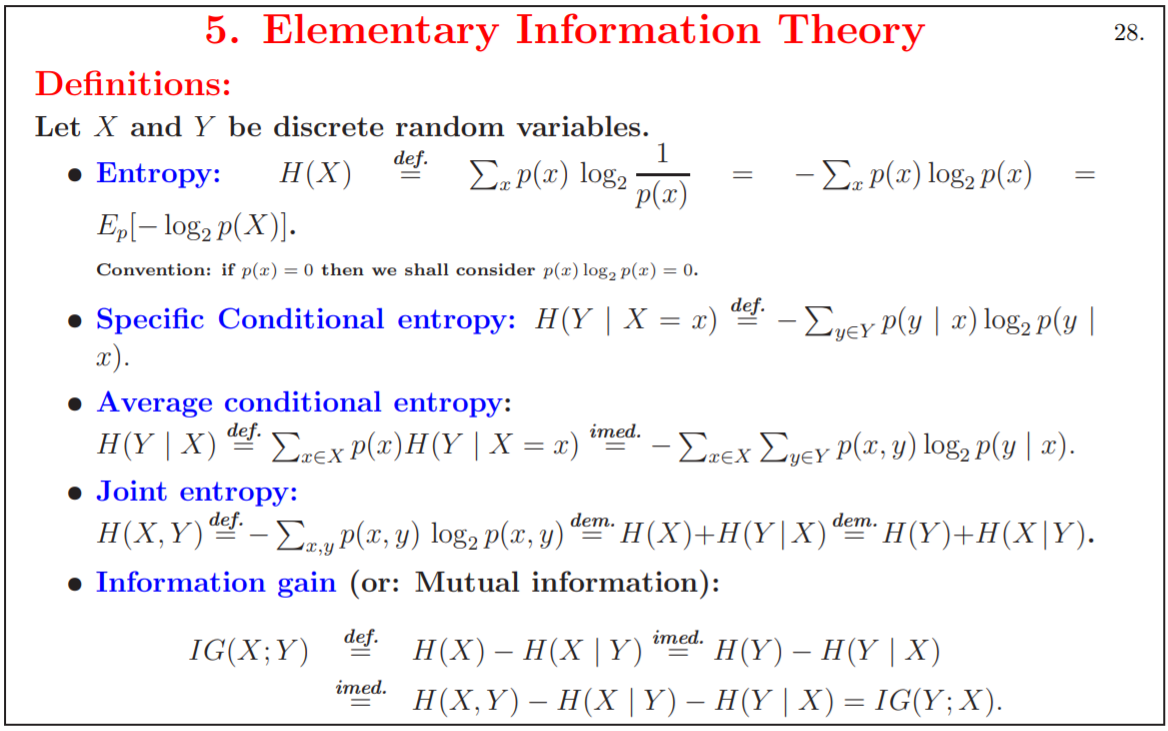
\includegraphics[width=1\linewidth]{D:/facultate/predat/2019-2020/fisiere/S3/screenshot043}
	\end{center}
	
	\begin{center}
		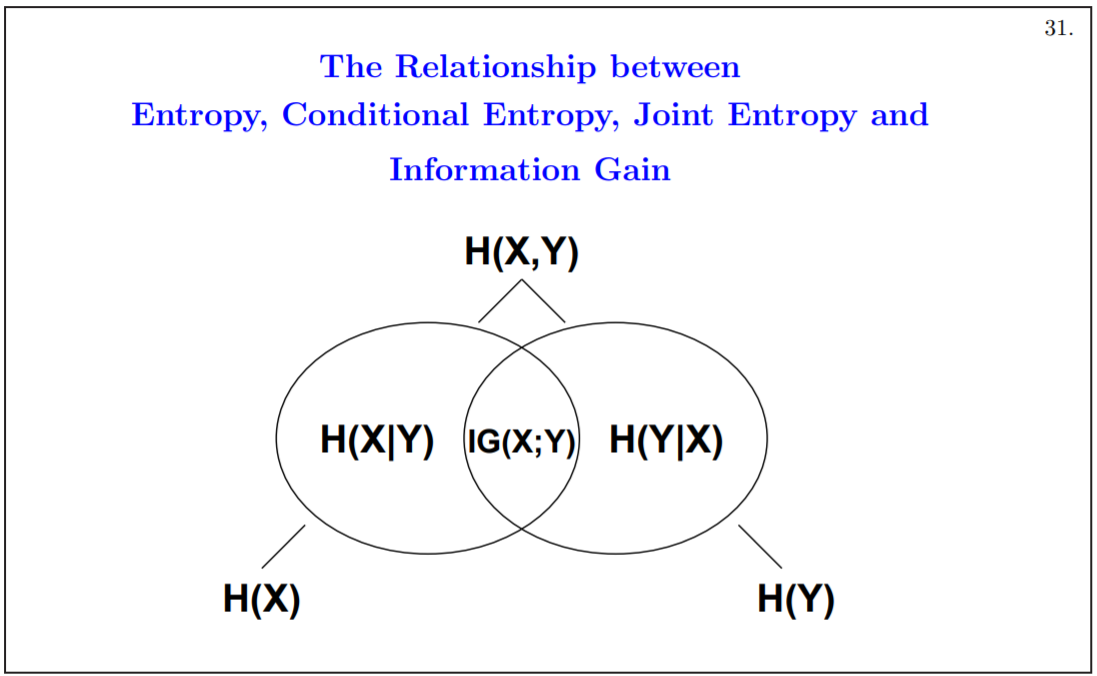
\includegraphics[width=1\linewidth]{D:/facultate/predat/2019-2020/fisiere/S3/screenshot044}
	\end{center}
	(slide-uri preluate din \url{https://profs.info.uaic.ro/~ciortuz/SLIDES/foundations.pdf})
	
	\newpage
	
	\textbf{Intuiții / Observații}:
	\begin{enumerate}
		\item \textbf{Interpretări intuitive pentru entropie} ($H(X)$):
		\begin{enumerate}
			\item gradul mediu de
			\begin{itemize}
				\item surpriză
				\item incertitudine
			\end{itemize}
			\item cantitatea medie de informație
			\begin{itemize}
				\item pe care o conține $X$
				\item de care ai nevoie ca să-l afli pe $X$
				\item \textbf{necesară} pentru a-l afla pe $X$
			\end{itemize}
		\end{enumerate}
		\item \textbf{Entropia condițională specifică}: $H(Y|X=x)$
		\item \textbf{Entropia condițională medie}: $H(Y|X)$
		\begin{itemize}
			\item dacă în $H(X)$ și $H(Y|X=x)$, $X$ și $Y|X=x$ sunt niște variabile aleatore, în $H(Y|X)$, $Y|X$ nu este o variabilă aleatoare și de aceea, în definiția lui $H(Y|X)$, ideea este să se ajungă la variabile aleatore de tipul $H(Y|X=x)$ (vezi definiția lui $H(Y|X)$)
		\end{itemize}
		\item \textbf{Entropia corelată}: $H(X,Y)$
		\begin{itemize}
			\item aici, ca și la $H(X)$ și $H(Y|X=x)$, $(X,Y)$ este o variabilă aleatoare
			\item Se poate demonstra că $H(X,Y) = H(X) + H(Y|X)$, ceea ce, conform intuiției are loc:
			
			Pentru a afla (X,Y), să zicem că aflăm mai întâi pe X și apoi, după ce l-am aflat pe X, îl aflăm pe Y.
			
			(cantitatea medie de informație necesară pentru a afla pe (X,Y)) = (cantitatea medie de informație necesară pentru a afla pe X) + (știindu-l deja pe X, cantitatea medie de informație necesară pentru a afla pe Y)
		\end{itemize}
		\item \textbf{Câștigul de informație}: $IG(X;Y) \stackrel{\text{def.}}{=} H(X) - H(X|Y)$
		
		- se mai notează $IG(X|Y)$
		
		\textbf{	Intuiție
			\begin{itemize}
				\item context: pe $X$ nu-l știm, pe $Y$ îl știm
				\item $IG(X;Y)$ = dacă îl știm pe $Y$, câtă informație câștigăm în procesul de aflare a lui $X$ = (cantiatea medie de informație necesară pentru a-l afla pe X) - (știindu-l deja pe Y, cantitatea medie de informație pentru a-l afla pe X) = $H(X) - H(X|Y)$
		\end{itemize}}
		
		Este simetric: $IG(X;Y) = IG(Y;X)$.
		
		\item Am avut de-a face cu două tipuri de informație: 
		\begin{itemize}
			\item \textbf{informație necesară} (în cazul \textbf{entropiei})
			\item \textbf{informație câștigată} (în cazul \textbf{câștigului de informație})
		\end{itemize}
	\end{enumerate}
	
	\textbf{Proprietăți esențiale}:
	\begin{enumerate}
		\item $0 \leq H(X) \leq \log_2 |\text{Val}(X)|$
		
		Pentru distribuția Bernoulli (Val($X$) = \{0,1\}), avem: $0 \leq H(X) \leq \log_2 2 = 1$
		
		\textbf{Atenție: La exercițiile de la probabilități, știți că dacă la calcule vă dă o probabilitate mai mare decât 1 (sau negativă), atunci SIGUR ați greșit undeva. La fel și aici: dacă în calcule vă dă o entropie negativă sau mai mare decât poate ea să fie (de exemplu, mai mare decât 1 în cazul distribuției Bernoulli), atunci SIGUR ați greșit la calcule.}
		
		\item $IG(X;Y) \geq 0$
		
		\textbf{Atenție: Dacă, din calcule, obțineți un IG negativ, atunci SIGUR ați greșit undeva.}
	\end{enumerate}
	
	\newpage
	
	\textbf{\large{Am zis că facem PS. Am făcut probabilități. Urmează puțină, puțină:}}
	
	\textbf{\large{Statistică}}
	
	Până acum probabilitățile v-au fost date în exerciții, iar când nu au fost date în totalitate ați presupus voi echiprobabilitate sau independență.
	
	Să zicem că vă dau în mână o monedă. Cum faceți ca să aflați probabilitatea să cadă heads, pentru moneda aceasta?
	
	Posibil răspuns: 
	\begin{itemize}
		\item aruncăm moneda de mai multe ori
		\item reținem datele (adică ce a căzut la fiecare aruncare)
		\item asignăm probabilitățile
	\end{itemize}
	
	De exemplu: să zicem că ați aruncat moneda de 6 ori și ați obținut H, H, H, T, H, H. Care este probabilitatea să dea H (heads)? După cum intuiți:
	$$P(H) = \frac{5}{6}$$
	$$P(T) = \frac{1}{6}$$
	
	Ceea ce ați făcut se cheamă \textbf{estimare}: ați estimat probabilitățile din \textbf{date}. Mai mult, ați făcut o \textbf{estimare în sensul verosimilității maxime (\textit{maximum likelihood estimation}, MLE)}. La un moment, într-un seminar vom intra în detaliile acestui MLE, însă până atunci vreau să vă obișnuiți cu terminologia.
	
	\textit{Privire de ansamblu: am conectat lumea reală (practică) la teoria probabilităților (care este formală) prin statistică.}
	
	\textbf{Unde intervine statistica în ML? Mai țineți minte exemplul cu apartamentele de la primul seminar? }
	
	\begin{center}
		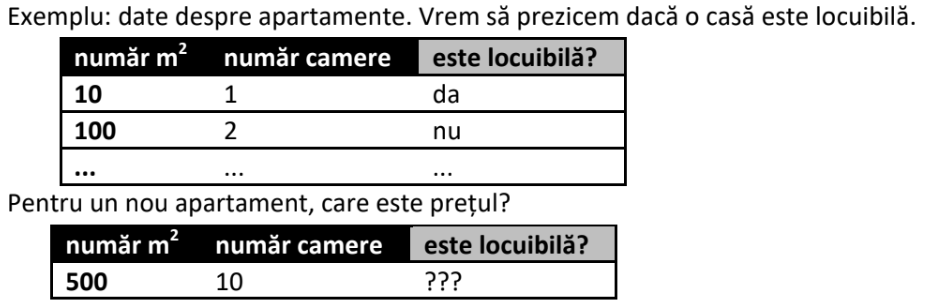
\includegraphics[width=\linewidth]{D:/facultate/predat/2019-2020/fisiere/S3/screenshot045}
	\end{center}
	\textbf{Dacă vreți, numele coloanelor (numar de m$^2$ etc.) sunt numele unor variabile aleatore, iar rândurile sunt de fapt realizări ale experimentului aleator (= ce s-a observat în urma experimentului aleator = date).}
	\\
	
	Ne vom întoarce puțin la entropii. Haideți să mai luăm un exemplu:
	Să zicem că datele, în urma repetării unui experiment de mai multe ori, sunt: 0,0,0,1,1,0. Putem estima probabilitățile în sensul verosimilității maxime (MLE):
	$$X:\begin{pmatrix}
	0 & 1\\
	\frac{4}{6} & \frac{2}{6}
	\end{pmatrix}$$
	Haideți să calculăm entropia lui $X$.
	$$H(X) = \frac{4}{6} \log_2 \frac{6}{4} + \frac{2}{6} \log_2 \frac{6}{2} = 0.9182$$
	Pentru a sări acești pași intermediari atunci când dorim să calculăm entropii, oamenii s-au gândit să inventeze ideea de \textbf{entropie a unui set de date}. În cazul nostru: 
	$$H[\text{date}] = H[0,0,0,1,1,0] \stackrel{\text{reetchetând:}0\rightarrow -, 1\rightarrow +}{=} = H[-,-,-,+,+,-] = H[2+,4-] \stackrel{\text{not.}}{=} H(X)$$
	Așadar, dacă vi se cerea să calculați entropia setului de date 0,0,0,1,1,0, puteți scrie direct că este
	$$H[2+,4-] = \frac{2}{2+4} \log_2 \frac{2+4}{2} + \frac{4}{2+4} \log_2 \frac{2+4}{4} = 0.9182$$
	
	În plus, mai observăm că $H[0+,6-]=0$ și $H[3+,3-]=1$.
	
	\textbf{Astfel, reiese o nouă interpretare pentru entropie (aplicată direct pe date):
		gradul mediu de impuritate/dezordine pentru un set de date.}
	
	\newpage
	
	\textbf{\large{Învățare automată supervizată de tip clasificare}}
	
	Dacă vă amintiți exemplul cu apartamentele de la primul seminar:
	\begin{center}
		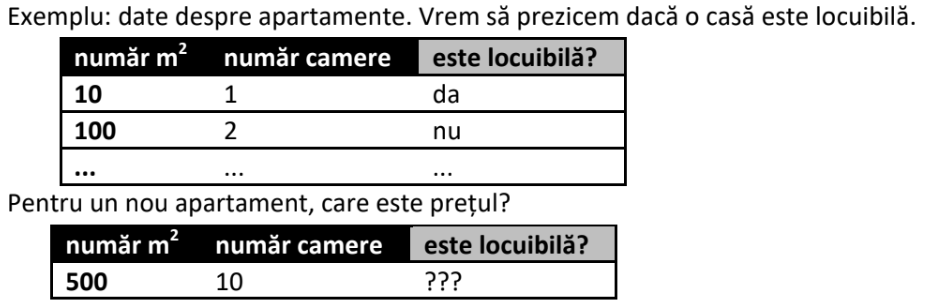
\includegraphics[width=\linewidth]{D:/facultate/predat/2019-2020/fisiere/S3/screenshot045}
	\end{center}
	mai știți că v-am zis că 
	\begin{itemize}
		\item primele două \textbf{coloane/atribute} sunt \textbf{de intrare}
		\item ultima coloană/ultimul atribut este \textbf{de ieșire}
		\item rândurile se mai cheamă \textbf{observații/instanțe}
		\item dorim să dăm unui algoritm primul tabel ca să învețe/se antreneze, iar apoi, după ce a învățat/s-a antrenat, (acest \textbf{algoritm} se cheamă \textbf{de antrenare}, iar primul tabel reprezintă \textbf{datele de antrenare})
		\item dăm unui al doilea algoritm al doilea tabel (care poate avea mai multe rănduri, nu doar unul ca în exemplu; de obicei, deși nu obligatoriu, vor fi rânduri nemaivăzute de algoritm la antrenare), iar algoritmul ne va furniza pentru fiecare rând din tabelul al doilea câte o valoare (etichetă) pentru coloana necunoscută (acest \textbf{algoritm} se cheamă \textbf{de testare}, iar al doilea tabel reprezintă \textbf{datele de testare})
		\item spunem că algoritmul de antrenare furnizează un \textbf{model/parametrii unui model} (exemple: arbore, parametrii unei distribuții de probabilitate etc.)
	\end{itemize}  
	Programatic, codul \textit{high-level} ar suna astfel:
	\begin{verbatim}
	model = trainingAlgorithm(trainingData)
	predictedLabels = testingAlgorithm(model, testingData)
	\end{verbatim}
	
	Totuși, testingAlgorithm poate fi apelat și cu trainingData în loc de testingData și se pot compara etichetele corecte (cele din tabelul 1) cu cele furnizate de algoritm și se poate calcula o eroare:
	
	\textbf{Eroarea la antrenare} = $\frac{\text{numărul de rânduri etichetate greșit}}{\text{numărul de rânduri la antrenament}}$
	
	\textbf{Acuratețea la antrenare} = $\frac{\text{numărul de rânduri etichetate corect}}{\text{numărul de rânduri la antrenament}}$
	
	Deci, Eroarea la antrenare = 1 - Acuratețea la antrenare.
	
	Un \textbf{set de date este inconsistent} dacă în setul de date există (măcar) două rânduri care, pe atributele de intrare sunt identice, însă la ieșire ele diferă.
	
	\textbf{\large{Arbori de decizie}}
	
	Arbore cu:
	\begin{itemize}
		\item noduri
		\begin{itemize}
			\item interne/de test: nume de coloană/atribut/variabilă aleatoare de intrare
			\item frunză/de decizie: valoare a coloanei de ieșire
		\end{itemize}
		\item ramuri: valoare a nodului părinte
	\end{itemize}
	Care este algoritmul de testare pentru un arbore de decizie?
	Exemplu:
	
	\begin{center}
		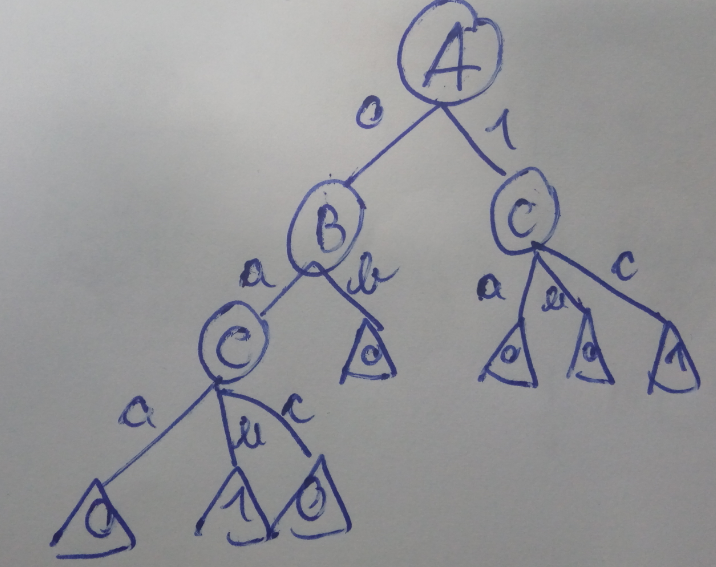
\includegraphics[width=0.7\linewidth]{D:/facultate/predat/2019-2020/fisiere/S3/screenshot046}
	\end{center}
	
	
	Pentru (A = 0, B = a, C = b) algoritmul va furniza 1.
	
	Pentru (A = 1, B = b, C = c) algoritmul va furniza 1.
	
	\textbf{\large{Algoritmul ID3}}
	
	- construiește un arbore de decizie
	
	- \textbf{bias-ul inductiv} (intuitiv = cum consideră algoritmul că ar trebui să prezicem coloana de ieșire) al algoritmului ID3: [dorim ca modelul să aibă structură ierarhică, să fie consistent cu datele dacă acestea sunt consistente, iar arborele ID3 trebuie să aibă un număr cât mai mic de niveluri/noduri
	(preluat din \url{https://profs.info.uaic.ro/~ciortuz/ML.ex-book/sumar.pdf})
	
	\textbf{Atenție: Algoritmul ID3 nu găsește arborele optimal din punctul de vedere al numărului de noduri/niveluri, ci doar încearcă să-l găsească.}
	
	Pentru detalii vedeți ex. 2/pag. 263.
	
	Apoi urmăriți cum se construiește arborele de la ex. 4/pag. 270 și citiți și observațiile următoare.
	
	Observații de urmărit odată cu exercițiul 4:
	\begin{enumerate}
		\item Normal, când se alege un atribut de intrare pentru a fi așezat într-un nod, se calculează IG-uri și se alege atributul cu IG-ul maxim. În problema dată, nu se calculează IG-uri, ci entropii condiționale medii și se alege atributul cu entropia (cond. medie) minimă, ceea ce are sens. (Dacă ai citit până aici, vreau să intri pe site-ul seminarului. Pe prima pagină ai un link pentru feedback anonim. Intră acolo și scrie "Am citit". Vreau să-mi fac o idee cam câți citesc. Mersi.) De exemplu, pentru rădăcină, în loc să se calculeze
		$$IG_{0/A} = H_0 - H_{0/A}$$
		$$IG_{0/B} = H_0 - H_{0/B}$$
		$$IG_{0/C} = H_0 - H_{0/C}$$
		și să se aleagă atributul (A, B sau C) cu IG-ul maxim, se calculează doar 
		$$H_{0/A}$$
		$$H_{0/B}$$
		$$H_{0/C}$$
		și se alege atributul (A, B sau C) după H-ul minim, pentru a scăpa de niște calcule. Acest lucru este posibil pentru că $H_0$ apare în toate cele 3 IG-uri...
		
		\item Există următoarea notație: 
		$$IG_\text{\#nod/atribut intrare} = H_\text{\#nod} - H_\text{\#nod/atribut intrare}$$
		care înseamnă
		$$IG_{(Y|\dots);(\text{atribut intrare}|\dots)} = H_{Y|\dots} - H_{(Y|\dots)|(\text{atribut intrare}|\dots)}$$
		
		De exemplu, în exercițiu, avem:
		$$IG_{0/A} = H_0 - H_{0/A}$$
		care înseamnă
		$$IG_{Y;A} = H_Y - H_{Y|A}$$
		și 
		$$IG_{1/A} = H_1 - H_{1/A}$$
		care înseamnă
		$$IG_{(Y|C=1);(A|C=1)} = H_{Y|C=1} - H_{(Y|C=1)|(A|C=1)}$$
		
		\item Un atribut poate apărea de mai multe ori în arbore, DAR doar o singură dată pe un drum de la rădăcină la o frunză.
		
		\item Condiții de oprire ID3
		\begin{itemize}
			\item nu mai există atribute pe care să le punem în nodurile de test (toate atributele se află pe drumul de la actualul nod la rădăcină)
			\item toate nodurile sunt pure (adică, de tipul [2+,0-],[0+,10-], [3a,0b,0c] etc.)
		\end{itemize}
	\end{enumerate}
	
	Observație: Când rezolvați exerciții, urmăriți \textit{Proprietățile numerice / calitative ale arborilor ID3} din Sumar (pagina 11 - \url{https://profs.info.uaic.ro/~ciortuz/ML.ex-book/sumar.pdf}). 
	
	\newpage
	\textbf{\large{Schemă de final}}
	\begin{enumerate}
		\item Teoria informației
		\begin{enumerate}
			\item Entropie
			\begin{enumerate}
				\item definiție
				\item interpretări (informație necesară)
				\item entropie condițională specifică
				\item entropie condițională medie
				\item entropie corelată
				\item $0 \leq H(X) \leq \log_2|\text{Val}(X)|$
			\end{enumerate}
			\item Câștig de informație
			\begin{enumerate}
				\item definiție
				\item interpretări (informație câștigată)
				\item $IG(X;Y) \geq 0$
			\end{enumerate}
		\end{enumerate}
		\item Statistică
		\begin{enumerate}
			\item date
			\item estimare
			\begin{enumerate}
				\item estimare în sensul verosimilității maxime (MLE)
			\end{enumerate}
			\item entropia unui set de date
		\end{enumerate}
		\item Învățare supervizată de tip clasificare
		\begin{enumerate}
			\item arbori de decizie
			\begin{enumerate}
				\item algoritmul ID3
			\end{enumerate}
		\end{enumerate}
	\end{enumerate}
	
\end{document}